\documentclass{article}
\usepackage[T1]{fontenc}
\usepackage{lmodern}
\usepackage{graphicx}
\usepackage{amsmath,amssymb}
\usepackage[a4paper,margin=2cm]{geometry}
\usepackage[absolute,overlay]{textpos}
\setlength{\TPHorizModule}{1mm}
\setlength{\TPVertModule}{1mm}
\usepackage[indonesian]{babel}
\usepackage{hyperref}
\setlength{\emergencystretch}{2em}
% unit: Halaman 41

\begin{document}

% === Halaman 41 (llm) ===

% (tidak ada teks dari model)

% deskripsi: Screenshot kode program Python untuk menghasilkan kunci RSA menggunakan library Crypto.PublicKey dengan parameter e = 97 dan panjang kunci 2048 bit, serta menampilkan hasil nilai e dan d.
% bbox normalisasi: [0.0000, 0.1700, 1.0000, 0.7200]
\begin{textblock*}{210.00mm}(0.00mm,50.49mm)
\noindent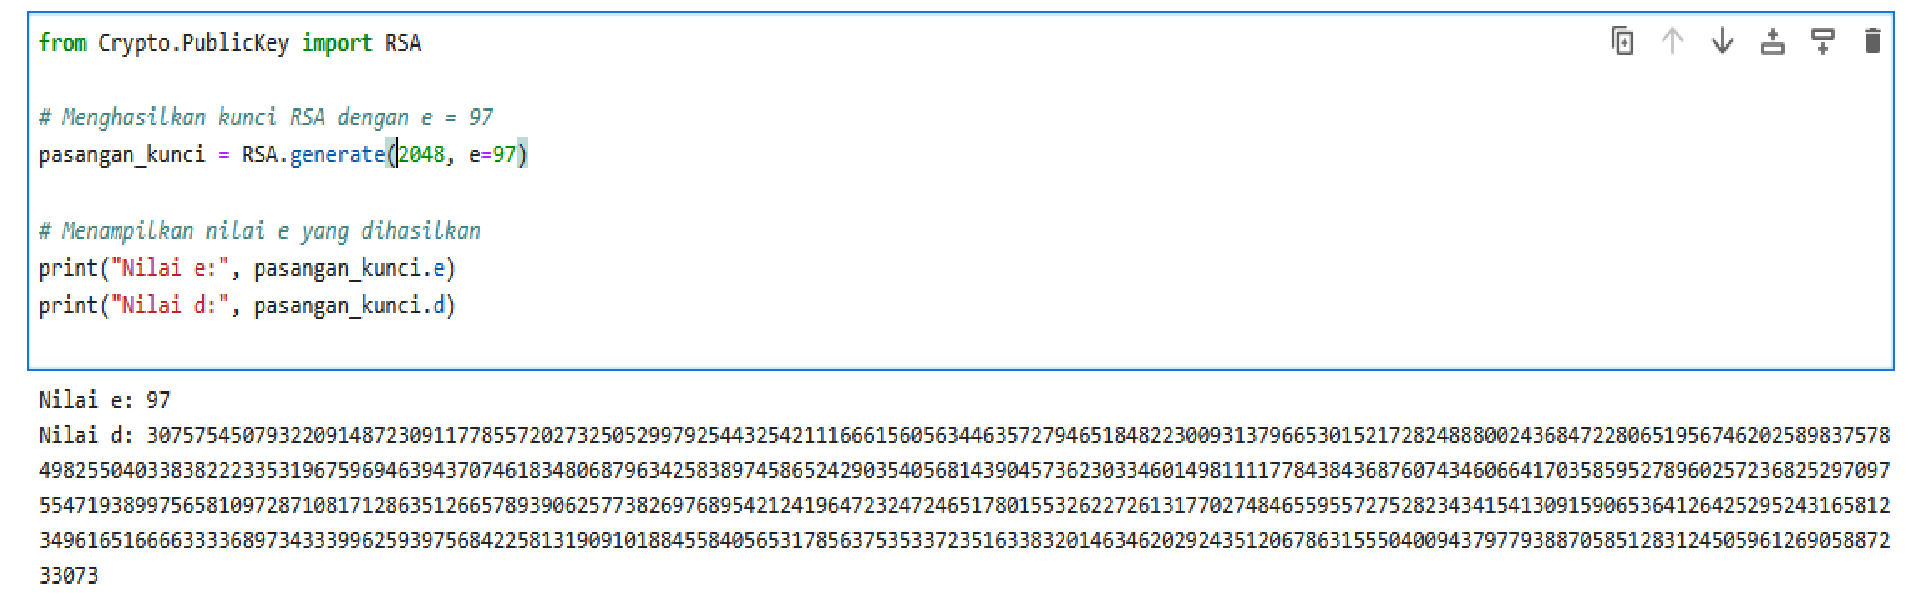
\includegraphics[width=210.00mm,height=163.35mm]{../../images/llm/page_041_img_01.png}%
\end{textblock*}

\end{document}
